\documentclass[14pt]{extbook}
\usepackage{multicol, enumerate, enumitem, hyperref, color, soul, setspace, parskip, fancyhdr} %General Packages
\usepackage{amssymb, amsthm, amsmath, latexsym, units, mathtools} %Math Packages
\everymath{\displaystyle} %All math in Display Style
% Packages with additional options
\usepackage[headsep=0.5cm,headheight=12pt, left=1 in,right= 1 in,top= 1 in,bottom= 1 in]{geometry}
\usepackage[usenames,dvipsnames]{xcolor}
\usepackage{dashrule}  % Package to use the command below to create lines between items
\newcommand{\litem}[1]{\item#1\hspace*{-1cm}\rule{\textwidth}{0.4pt}}
\pagestyle{fancy}
\lhead{Progress Quiz 9}
\chead{}
\rhead{Version ALL}
\lfoot{9541-5764}
\cfoot{}
\rfoot{Summer C 2021}
\begin{document}

\begin{enumerate}
\litem{
Solve the rational equation below. Then, choose the interval(s) that the solution(s) belongs to.\[ \frac{-30}{35x -10} + 1 = \frac{-30}{35x -10} \]\begin{enumerate}[label=\Alph*.]
\item \( x \in [0.29,2.29] \)
\item \( \text{All solutions lead to invalid or complex values in the equation.} \)
\item \( x \in [-0.4,0.2] \)
\item \( x_1 \in [-0.4, 0.2] \text{ and } x_2 \in [-0.71,2.29] \)
\item \( x_1 \in [0.2, 0.8] \text{ and } x_2 \in [-0.71,2.29] \)

\end{enumerate} }
\litem{
Choose the graph of the equation below.\[ f(x) = \frac{1}{(x - 2)^2} - 2 \]\begin{enumerate}[label=\Alph*.]
\begin{multicols}{2}\item 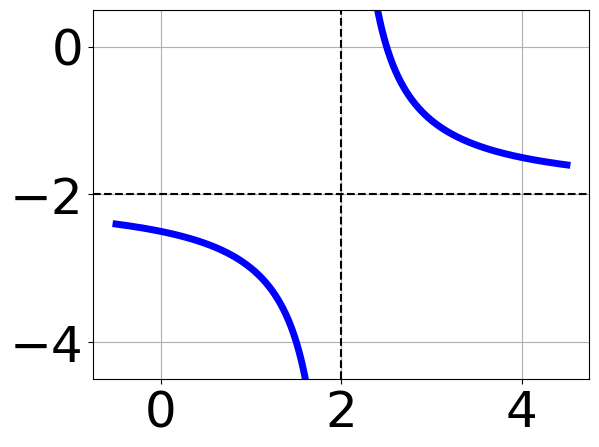
\includegraphics[width = 0.3\textwidth]{../Figures/rationalEquationToGraphCopyAA.png}\item 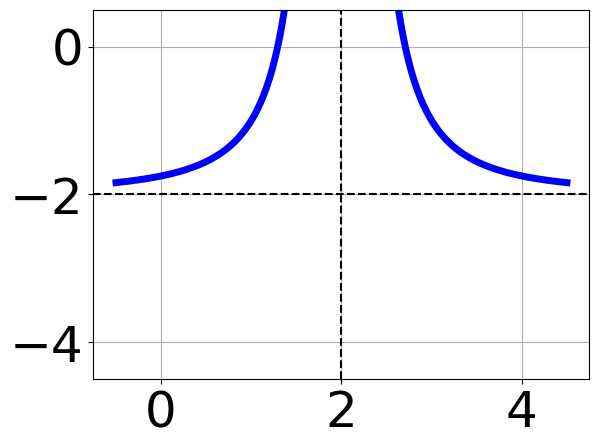
\includegraphics[width = 0.3\textwidth]{../Figures/rationalEquationToGraphCopyBA.png}\item 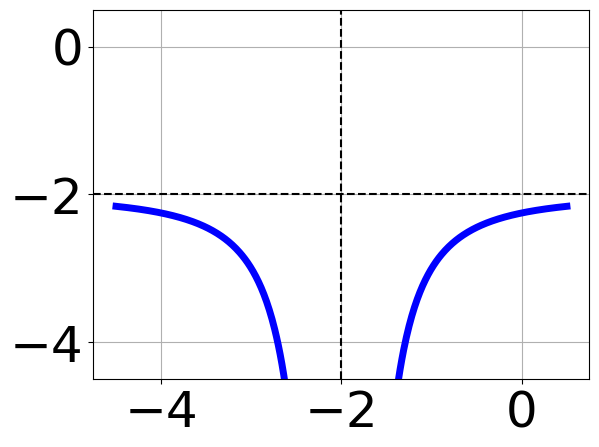
\includegraphics[width = 0.3\textwidth]{../Figures/rationalEquationToGraphCopyCA.png}\item 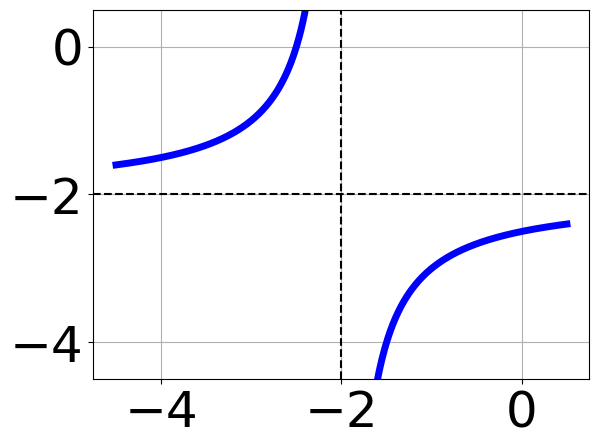
\includegraphics[width = 0.3\textwidth]{../Figures/rationalEquationToGraphCopyDA.png}\end{multicols}\item None of the above.
\end{enumerate} }
\litem{
Solve the rational equation below. Then, choose the interval(s) that the solution(s) belongs to.\[ \frac{2x}{7x + 2} + \frac{-5x^{2}}{-35x^{2} -31 x -6} = \frac{4}{-5x -3} \]\begin{enumerate}[label=\Alph*.]
\item \( x \in [-0.53,0.55] \)
\item \( \text{All solutions lead to invalid or complex values in the equation.} \)
\item \( x_1 \in [-2.69, -1.04] \text{ and } x_2 \in [-0.27,-0.24] \)
\item \( x \in [-0.88,-0.31] \)
\item \( x_1 \in [-2.69, -1.04] \text{ and } x_2 \in [-0.3,-0.28] \)

\end{enumerate} }
\litem{
Determine the domain of the function below.\[ f(x) = \frac{6}{36x^{2} +54 x + 20} \]\begin{enumerate}[label=\Alph*.]
\item \( \text{All Real numbers except } x = a, \text{ where } a \in [-30.08, -29.84] \)
\item \( \text{All Real numbers.} \)
\item \( \text{All Real numbers except } x = a \text{ and } x = b, \text{ where } a \in [-0.86, -0.73] \text{ and } b \in [-0.73, -0.5] \)
\item \( \text{All Real numbers except } x = a, \text{ where } a \in [-0.86, -0.73] \)
\item \( \text{All Real numbers except } x = a \text{ and } x = b, \text{ where } a \in [-30.08, -29.84] \text{ and } b \in [-24.13, -23.8] \)

\end{enumerate} }
\litem{
Solve the rational equation below. Then, choose the interval(s) that the solution(s) belongs to.\[ \frac{-9}{4x -4} + -6 = \frac{-6}{-20x + 20} \]\begin{enumerate}[label=\Alph*.]
\item \( x_1 \in [-3.42, 0.57] \text{ and } x_2 \in [0.49,0.7] \)
\item \( x \in [-3.42,0.57] \)
\item \( x_1 \in [0.57, 3.58] \text{ and } x_2 \in [0.74,1.39] \)
\item \( \text{All solutions lead to invalid or complex values in the equation.} \)
\item \( x \in [0.57,1.57] \)

\end{enumerate} }
\litem{
Choose the equation of the function graphed below.
\begin{center}
    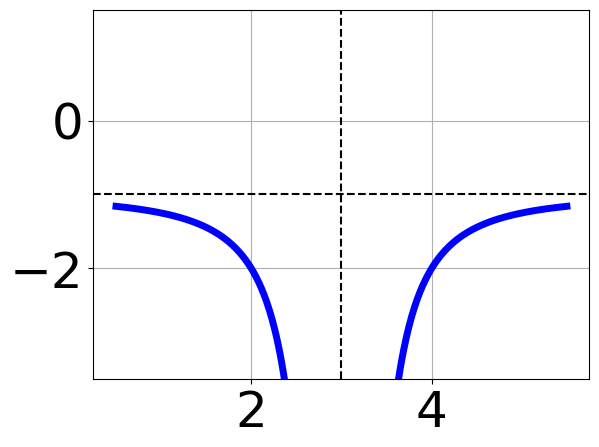
\includegraphics[width=0.5\textwidth]{../Figures/rationalGraphToEquationA.png}
\end{center}
\begin{enumerate}[label=\Alph*.]
\item \( f(x) = \frac{-1}{(x - 3)^2} - 1 \)
\item \( f(x) = \frac{1}{(x + 3)^2} - 1 \)
\item \( f(x) = \frac{1}{x + 3} - 1 \)
\item \( f(x) = \frac{-1}{x - 3} - 1 \)
\item \( \text{None of the above} \)

\end{enumerate} }
\litem{
Solve the rational equation below. Then, choose the interval(s) that the solution(s) belongs to.\[ \frac{-3x}{-6x -7} + \frac{-6x^{2}}{-30x^{2} -47 x -14} = \frac{-3}{5x + 2} \]\begin{enumerate}[label=\Alph*.]
\item \( x_1 \in [-1.64, -0.93] \text{ and } x_2 \in [-0.7,1.1] \)
\item \( x \in [-1.64,-0.93] \)
\item \( x \in [-0.54,-0.38] \)
\item \( \text{All solutions lead to invalid or complex values in the equation.} \)
\item \( x_1 \in [-0.6, -0.44] \text{ and } x_2 \in [-3.7,-1.3] \)

\end{enumerate} }
\litem{
Choose the graph of the equation below.\[ f(x) = \frac{-1}{(x - 3)^2} - 2 \]\begin{enumerate}[label=\Alph*.]
\begin{multicols}{2}\item 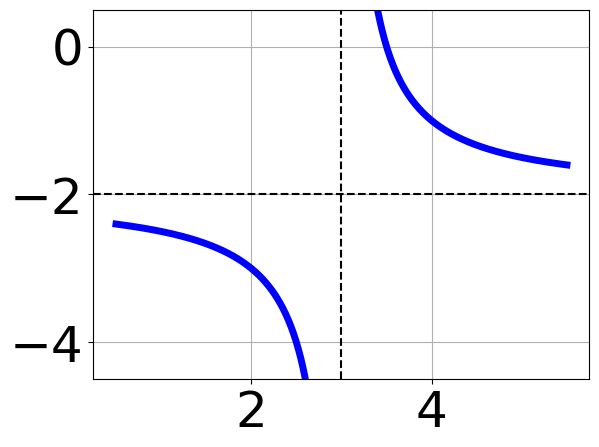
\includegraphics[width = 0.3\textwidth]{../Figures/rationalEquationToGraphAA.png}\item 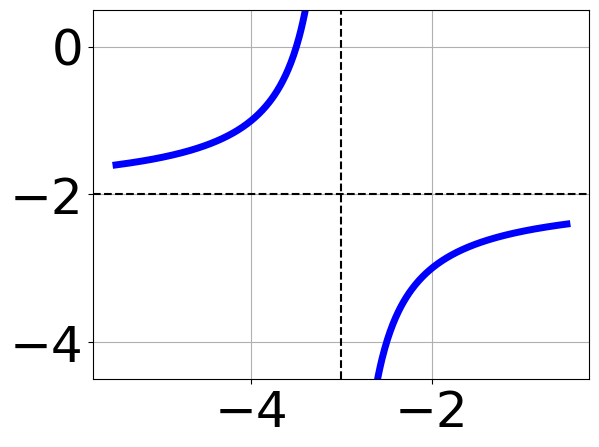
\includegraphics[width = 0.3\textwidth]{../Figures/rationalEquationToGraphBA.png}\item 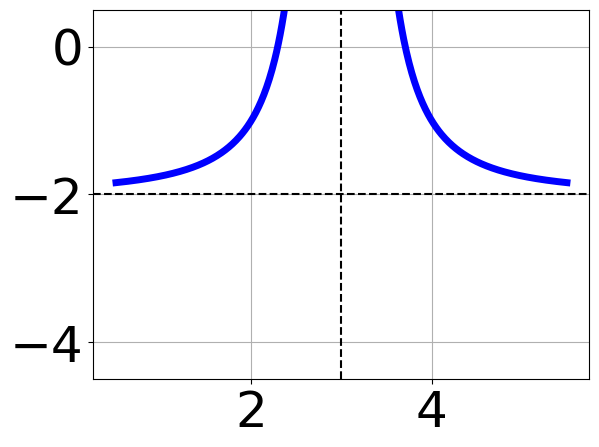
\includegraphics[width = 0.3\textwidth]{../Figures/rationalEquationToGraphCA.png}\item 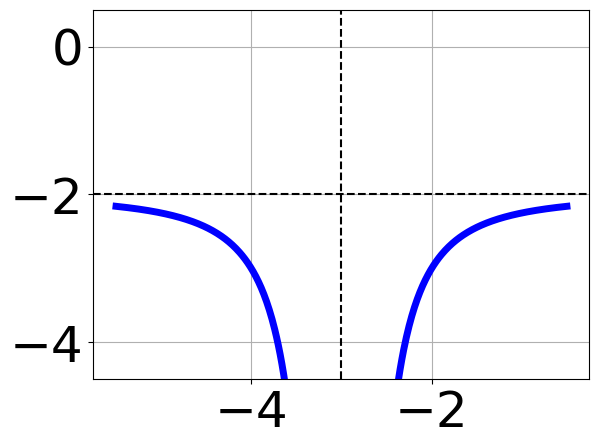
\includegraphics[width = 0.3\textwidth]{../Figures/rationalEquationToGraphDA.png}\end{multicols}\item None of the above.
\end{enumerate} }
\litem{
Choose the equation of the function graphed below.
\begin{center}
    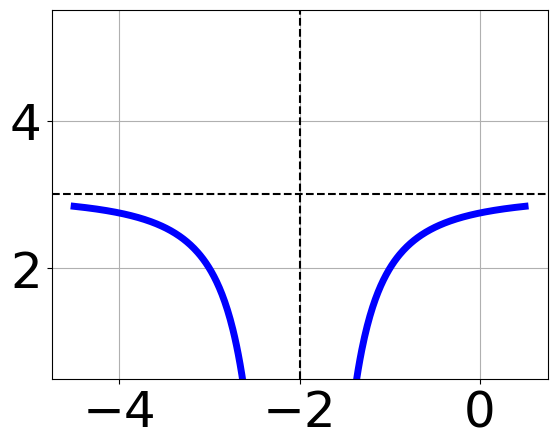
\includegraphics[width=0.5\textwidth]{../Figures/rationalGraphToEquationCopyA.png}
\end{center}
\begin{enumerate}[label=\Alph*.]
\item \( f(x) = \frac{-1}{(x + 2)^2} + 3 \)
\item \( f(x) = \frac{1}{x - 2} + 3 \)
\item \( f(x) = \frac{1}{(x - 2)^2} + 3 \)
\item \( f(x) = \frac{-1}{x + 2} + 3 \)
\item \( \text{None of the above} \)

\end{enumerate} }
\litem{
Determine the domain of the function below.\[ f(x) = \frac{5}{15x^{2} +42 x + 24} \]\begin{enumerate}[label=\Alph*.]
\item \( \text{All Real numbers except } x = a \text{ and } x = b, \text{ where } a \in [-20.36, -19.15] \text{ and } b \in [-18.44, -17.43] \)
\item \( \text{All Real numbers except } x = a, \text{ where } a \in [-2.3, -1.32] \)
\item \( \text{All Real numbers.} \)
\item \( \text{All Real numbers except } x = a, \text{ where } a \in [-20.36, -19.15] \)
\item \( \text{All Real numbers except } x = a \text{ and } x = b, \text{ where } a \in [-2.3, -1.32] \text{ and } b \in [-1, -0.34] \)

\end{enumerate} }
\litem{
Solve the rational equation below. Then, choose the interval(s) that the solution(s) belongs to.\[ \frac{4}{7x -5} + 3 = \frac{-3}{42x -30} \]\begin{enumerate}[label=\Alph*.]
\item \( x_1 \in [0.18, 0.4] \text{ and } x_2 \in [-0.5,2.5] \)
\item \( x \in [-1.11,-0.8] \)
\item \( \text{All solutions lead to invalid or complex values in the equation.} \)
\item \( x_1 \in [-1.11, -0.8] \text{ and } x_2 \in [-0.5,2.5] \)
\item \( x \in [-1.5,1.5] \)

\end{enumerate} }
\litem{
Choose the graph of the equation below.\[ f(x) = \frac{1}{(x + 3)^2} - 3 \]\begin{enumerate}[label=\Alph*.]
\begin{multicols}{2}\item 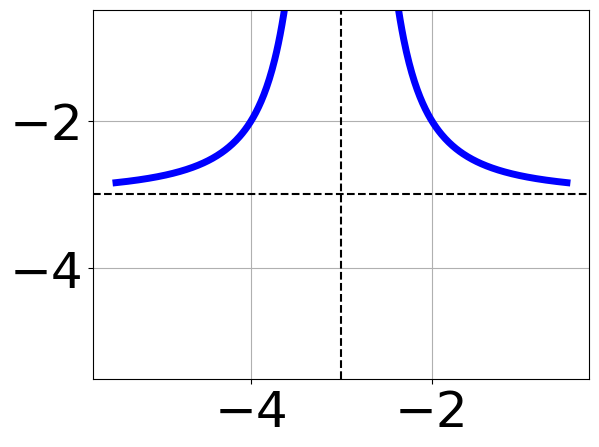
\includegraphics[width = 0.3\textwidth]{../Figures/rationalEquationToGraphCopyAB.png}\item 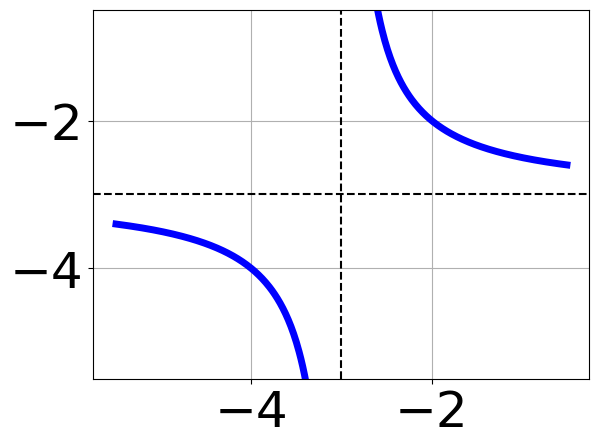
\includegraphics[width = 0.3\textwidth]{../Figures/rationalEquationToGraphCopyBB.png}\item 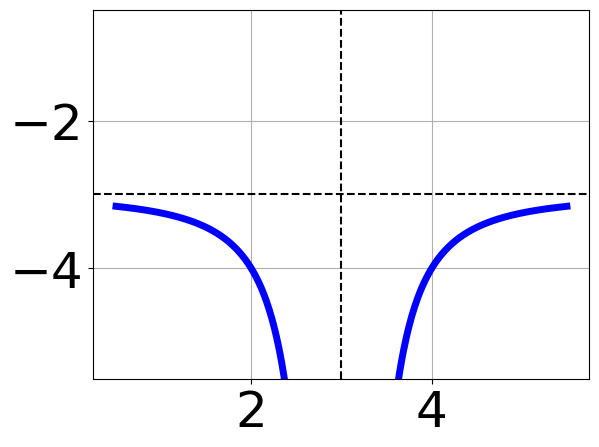
\includegraphics[width = 0.3\textwidth]{../Figures/rationalEquationToGraphCopyCB.png}\item 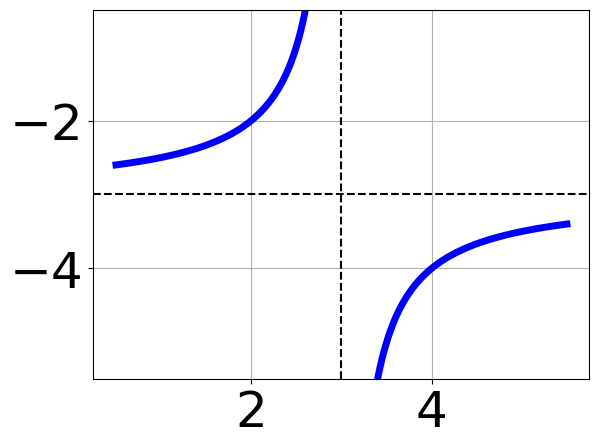
\includegraphics[width = 0.3\textwidth]{../Figures/rationalEquationToGraphCopyDB.png}\end{multicols}\item None of the above.
\end{enumerate} }
\litem{
Solve the rational equation below. Then, choose the interval(s) that the solution(s) belongs to.\[ \frac{3x}{-2x + 6} + \frac{-4x^{2}}{-8x^{2} +28 x -12} = \frac{-4}{4x -2} \]\begin{enumerate}[label=\Alph*.]
\item \( x_1 \in [-1.06, -0.31] \text{ and } x_2 \in [1.54,2.91] \)
\item \( \text{All solutions lead to invalid or complex values in the equation.} \)
\item \( x_1 \in [2.69, 3.2] \text{ and } x_2 \in [0.49,1.23] \)
\item \( x \in [0.38,1.49] \)
\item \( x \in [2.69,3.2] \)

\end{enumerate} }
\litem{
Determine the domain of the function below.\[ f(x) = \frac{5}{12x^{2} +2 x -24} \]\begin{enumerate}[label=\Alph*.]
\item \( \text{All Real numbers except } x = a, \text{ where } a \in [-1.5, -0.5] \)
\item \( \text{All Real numbers except } x = a, \text{ where } a \in [-24, -20] \)
\item \( \text{All Real numbers except } x = a \text{ and } x = b, \text{ where } a \in [-1.5, -0.5] \text{ and } b \in [-0.67, 2.33] \)
\item \( \text{All Real numbers except } x = a \text{ and } x = b, \text{ where } a \in [-24, -20] \text{ and } b \in [11, 13] \)
\item \( \text{All Real numbers.} \)

\end{enumerate} }
\litem{
Solve the rational equation below. Then, choose the interval(s) that the solution(s) belongs to.\[ \frac{-4}{-6x -5} + -8 = \frac{5}{-12x -10} \]\begin{enumerate}[label=\Alph*.]
\item \( x_1 \in [-0.7, 0.3] \text{ and } x_2 \in [-0.03,2.97] \)
\item \( x_1 \in [-0.7, 0.3] \text{ and } x_2 \in [-0.65,0.35] \)
\item \( \text{All solutions lead to invalid or complex values in the equation.} \)
\item \( x \in [-0.03,3.97] \)
\item \( x \in [-0.7,0.3] \)

\end{enumerate} }
\litem{
Choose the equation of the function graphed below.
\begin{center}
    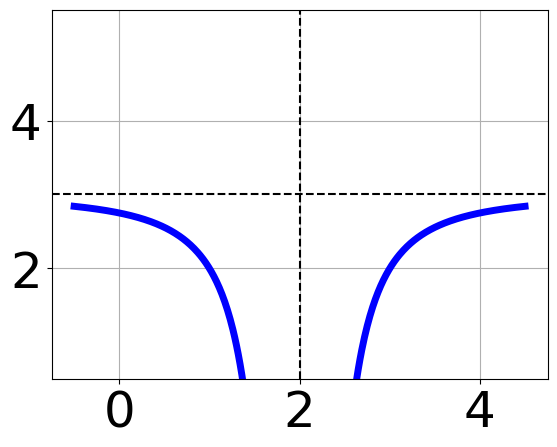
\includegraphics[width=0.5\textwidth]{../Figures/rationalGraphToEquationB.png}
\end{center}
\begin{enumerate}[label=\Alph*.]
\item \( f(x) = \frac{-1}{x - 2} + 3 \)
\item \( f(x) = \frac{1}{(x + 2)^2} + 3 \)
\item \( f(x) = \frac{-1}{(x - 2)^2} + 3 \)
\item \( f(x) = \frac{1}{x + 2} + 3 \)
\item \( \text{None of the above} \)

\end{enumerate} }
\litem{
Solve the rational equation below. Then, choose the interval(s) that the solution(s) belongs to.\[ \frac{-2x}{-4x -4} + \frac{-4x^{2}}{-20x^{2} -12 x + 8} = \frac{5}{5x -2} \]\begin{enumerate}[label=\Alph*.]
\item \( x \in [-0.13,0.5] \)
\item \( \text{All solutions lead to invalid or complex values in the equation.} \)
\item \( x_1 \in [-0.87, -0.46] \text{ and } x_2 \in [-3.5,-0.9] \)
\item \( x_1 \in [-0.87, -0.46] \text{ and } x_2 \in [1.8,3.3] \)
\item \( x \in [2.16,3.28] \)

\end{enumerate} }
\litem{
Choose the graph of the equation below.\[ f(x) = \frac{-1}{x + 1} + 3 \]\begin{enumerate}[label=\Alph*.]
\begin{multicols}{2}\item 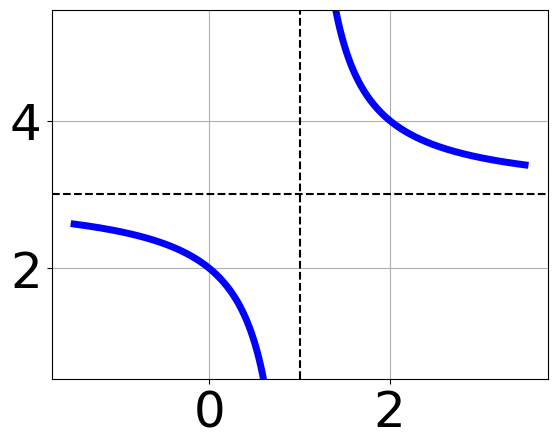
\includegraphics[width = 0.3\textwidth]{../Figures/rationalEquationToGraphAB.png}\item 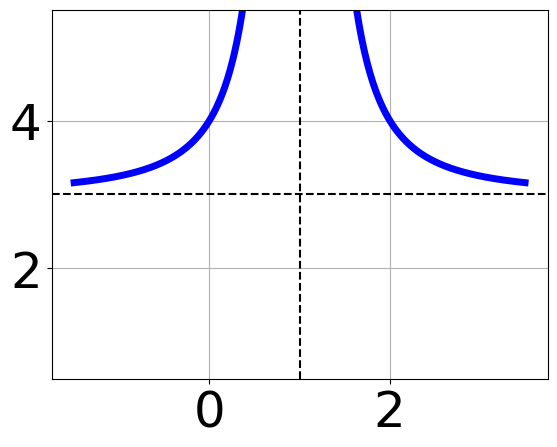
\includegraphics[width = 0.3\textwidth]{../Figures/rationalEquationToGraphBB.png}\item 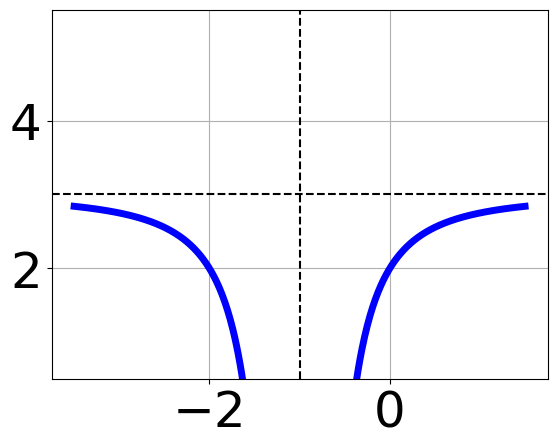
\includegraphics[width = 0.3\textwidth]{../Figures/rationalEquationToGraphCB.png}\item 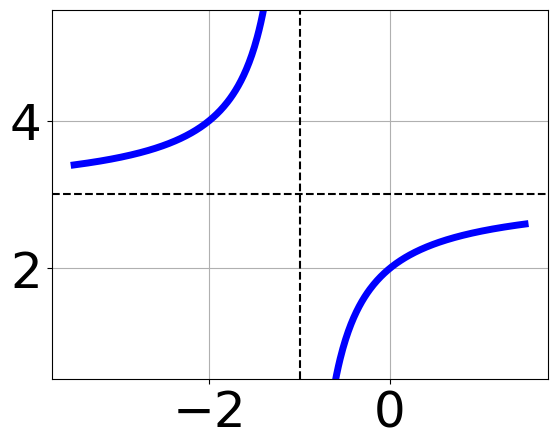
\includegraphics[width = 0.3\textwidth]{../Figures/rationalEquationToGraphDB.png}\end{multicols}\item None of the above.
\end{enumerate} }
\litem{
Choose the equation of the function graphed below.
\begin{center}
    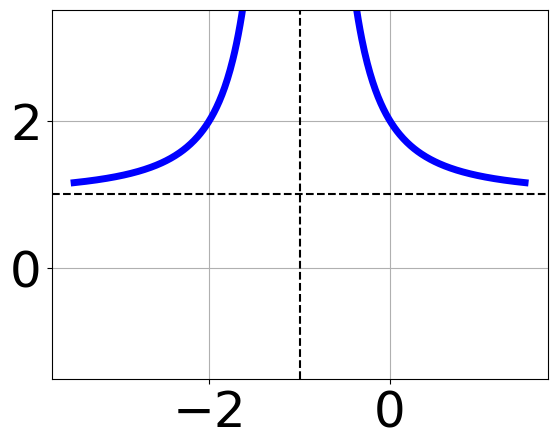
\includegraphics[width=0.5\textwidth]{../Figures/rationalGraphToEquationCopyB.png}
\end{center}
\begin{enumerate}[label=\Alph*.]
\item \( f(x) = \frac{1}{(x + 1)^2} + 1 \)
\item \( f(x) = \frac{1}{x + 1} + 1 \)
\item \( f(x) = \frac{-1}{x - 1} + 1 \)
\item \( f(x) = \frac{-1}{(x - 1)^2} + 1 \)
\item \( \text{None of the above} \)

\end{enumerate} }
\litem{
Determine the domain of the function below.\[ f(x) = \frac{6}{9x^{2} -25} \]\begin{enumerate}[label=\Alph*.]
\item \( \text{All Real numbers except } x = a, \text{ where } a \in [-4.67, 1.33] \)
\item \( \text{All Real numbers.} \)
\item \( \text{All Real numbers except } x = a \text{ and } x = b, \text{ where } a \in [-4.67, 1.33] \text{ and } b \in [-0.33, 3.67] \)
\item \( \text{All Real numbers except } x = a \text{ and } x = b, \text{ where } a \in [-16, -11] \text{ and } b \in [15, 20] \)
\item \( \text{All Real numbers except } x = a, \text{ where } a \in [-16, -11] \)

\end{enumerate} }
\litem{
Solve the rational equation below. Then, choose the interval(s) that the solution(s) belongs to.\[ \frac{-54}{-18x -36} + 1 = \frac{-54}{-18x -36} \]\begin{enumerate}[label=\Alph*.]
\item \( x_1 \in [-2, -1] \text{ and } x_2 \in [-3,-1] \)
\item \( \text{All solutions lead to invalid or complex values in the equation.} \)
\item \( x \in [0,3] \)
\item \( x_1 \in [-2, -1] \text{ and } x_2 \in [1,4] \)
\item \( x \in [-3.0,-1.0] \)

\end{enumerate} }
\litem{
Choose the graph of the equation below.\[ f(x) = \frac{1}{x - 3} - 1 \]\begin{enumerate}[label=\Alph*.]
\begin{multicols}{2}\item 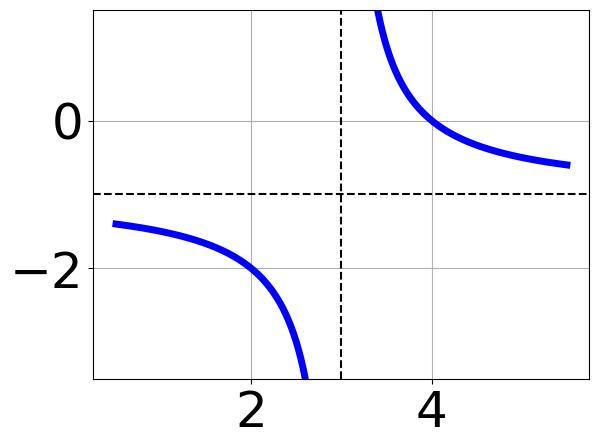
\includegraphics[width = 0.3\textwidth]{../Figures/rationalEquationToGraphCopyAC.png}\item 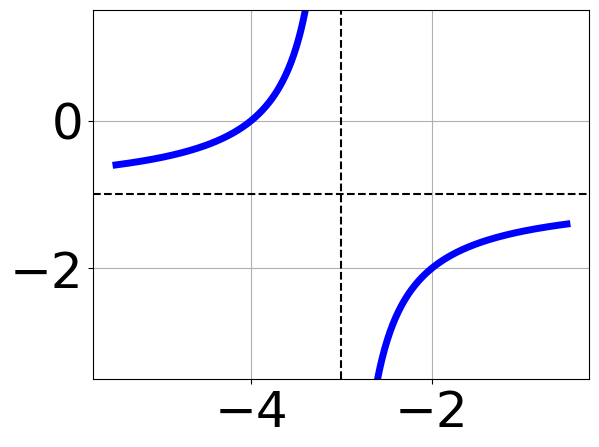
\includegraphics[width = 0.3\textwidth]{../Figures/rationalEquationToGraphCopyBC.png}\item 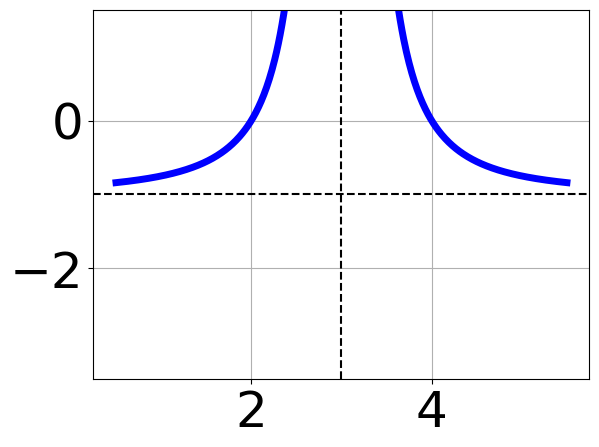
\includegraphics[width = 0.3\textwidth]{../Figures/rationalEquationToGraphCopyCC.png}\item 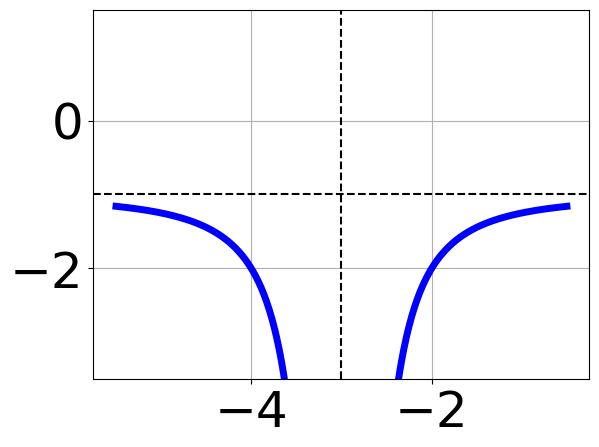
\includegraphics[width = 0.3\textwidth]{../Figures/rationalEquationToGraphCopyDC.png}\end{multicols}\item None of the above.
\end{enumerate} }
\litem{
Solve the rational equation below. Then, choose the interval(s) that the solution(s) belongs to.\[ \frac{7x}{2x -4} + \frac{-5x^{2}}{8x^{2} -20 x + 8} = \frac{4}{4x -2} \]\begin{enumerate}[label=\Alph*.]
\item \( \text{All solutions lead to invalid or complex values in the equation.} \)
\item \( x_1 \in [1.95, 3.73] \text{ and } x_2 \in [0.46,0.75] \)
\item \( x \in [0.03,1.35] \)
\item \( x \in [1.95,3.73] \)
\item \( x_1 \in [-1.93, -0.13] \text{ and } x_2 \in [0.71,1.15] \)

\end{enumerate} }
\litem{
Determine the domain of the function below.\[ f(x) = \frac{3}{18x^{2} +30 x + 12} \]\begin{enumerate}[label=\Alph*.]
\item \( \text{All Real numbers except } x = a, \text{ where } a \in [-1.93, -0.86] \)
\item \( \text{All Real numbers except } x = a \text{ and } x = b, \text{ where } a \in [-1.93, -0.86] \text{ and } b \in [-0.77, -0.49] \)
\item \( \text{All Real numbers.} \)
\item \( \text{All Real numbers except } x = a, \text{ where } a \in [-24.6, -23.08] \)
\item \( \text{All Real numbers except } x = a \text{ and } x = b, \text{ where } a \in [-24.6, -23.08] \text{ and } b \in [-9.56, -8.05] \)

\end{enumerate} }
\litem{
Solve the rational equation below. Then, choose the interval(s) that the solution(s) belongs to.\[ \frac{7}{-6x + 9} + 3 = \frac{-8}{-18x + 27} \]\begin{enumerate}[label=\Alph*.]
\item \( x_1 \in [-2.96, 1.04] \text{ and } x_2 \in [1.98,2.19] \)
\item \( x_1 \in [0.04, 4.04] \text{ and } x_2 \in [2.32,2.41] \)
\item \( x \in [-2.96,1.04] \)
\item \( \text{All solutions lead to invalid or complex values in the equation.} \)
\item \( x \in [2.04,3.04] \)

\end{enumerate} }
\litem{
Choose the equation of the function graphed below.
\begin{center}
    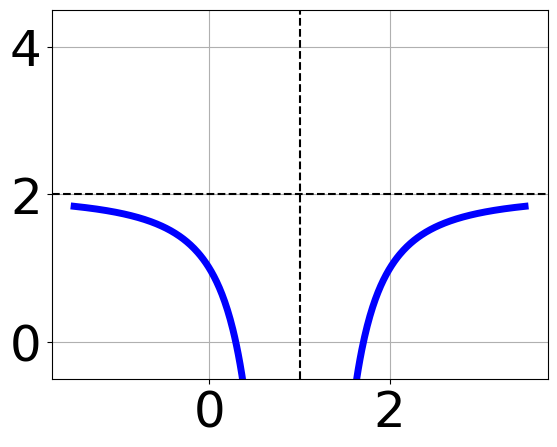
\includegraphics[width=0.5\textwidth]{../Figures/rationalGraphToEquationC.png}
\end{center}
\begin{enumerate}[label=\Alph*.]
\item \( f(x) = \frac{1}{(x + 1)^2} + 4 \)
\item \( f(x) = \frac{-1}{x - 1} + 4 \)
\item \( f(x) = \frac{-1}{(x - 1)^2} + 4 \)
\item \( f(x) = \frac{1}{x + 1} + 4 \)
\item \( \text{None of the above} \)

\end{enumerate} }
\litem{
Solve the rational equation below. Then, choose the interval(s) that the solution(s) belongs to.\[ \frac{6x}{7x + 6} + \frac{-3x^{2}}{49x^{2} +70 x + 24} = \frac{-2}{7x + 4} \]\begin{enumerate}[label=\Alph*.]
\item \( x \in [-0.9,-0.81] \)
\item \( \text{All solutions lead to invalid or complex values in the equation.} \)
\item \( x_1 \in [-0.9, -0.81] \text{ and } x_2 \in [-0.6,-0.54] \)
\item \( x \in [-0.64,-0.57] \)
\item \( x_1 \in [-0.8, -0.64] \text{ and } x_2 \in [-0.27,0.37] \)

\end{enumerate} }
\litem{
Choose the graph of the equation below.\[ f(x) = \frac{-1}{(x + 1)^2} - 2 \]\begin{enumerate}[label=\Alph*.]
\begin{multicols}{2}\item 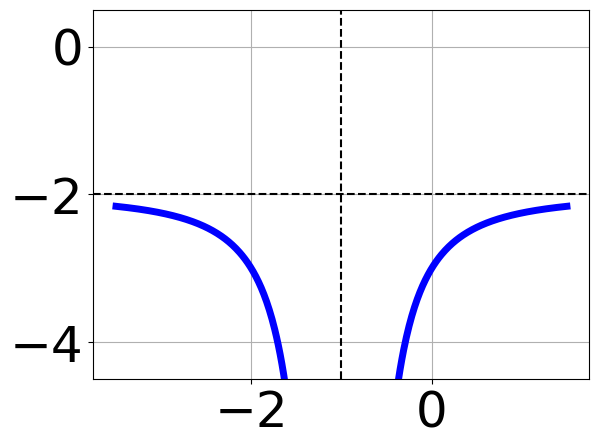
\includegraphics[width = 0.3\textwidth]{../Figures/rationalEquationToGraphAC.png}\item 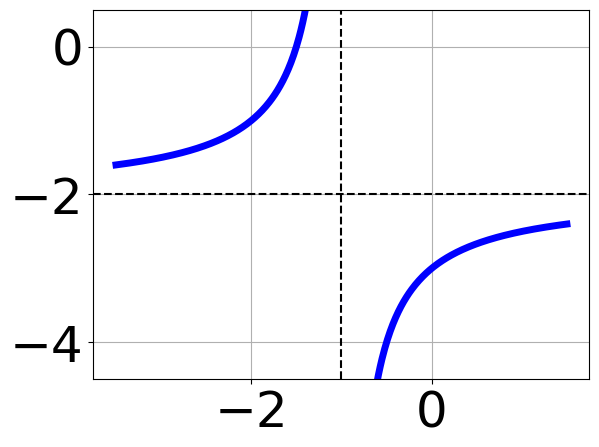
\includegraphics[width = 0.3\textwidth]{../Figures/rationalEquationToGraphBC.png}\item 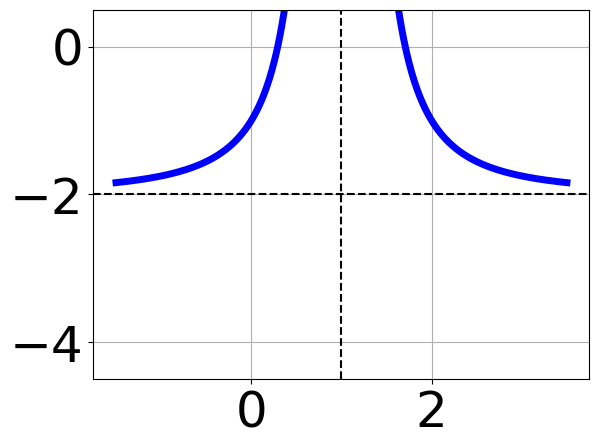
\includegraphics[width = 0.3\textwidth]{../Figures/rationalEquationToGraphCC.png}\item 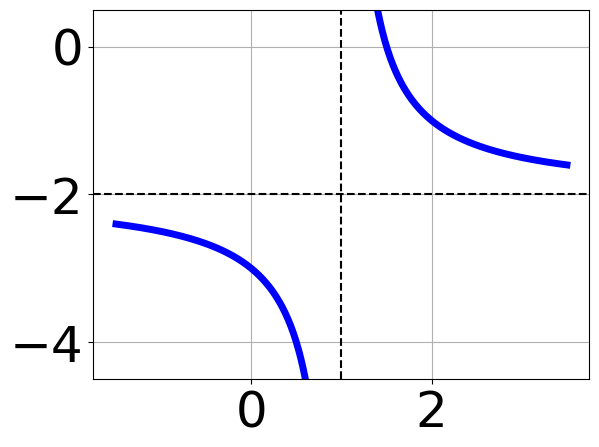
\includegraphics[width = 0.3\textwidth]{../Figures/rationalEquationToGraphDC.png}\end{multicols}\item None of the above.
\end{enumerate} }
\litem{
Choose the equation of the function graphed below.
\begin{center}
    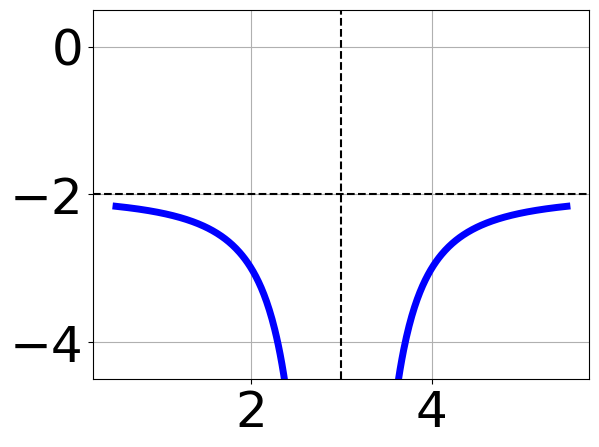
\includegraphics[width=0.5\textwidth]{../Figures/rationalGraphToEquationCopyC.png}
\end{center}
\begin{enumerate}[label=\Alph*.]
\item \( f(x) = \frac{-1}{x - 3} - 2 \)
\item \( f(x) = \frac{-1}{(x - 3)^2} - 2 \)
\item \( f(x) = \frac{1}{x + 3} - 2 \)
\item \( f(x) = \frac{1}{(x + 3)^2} - 2 \)
\item \( \text{None of the above} \)

\end{enumerate} }
\litem{
Determine the domain of the function below.\[ f(x) = \frac{4}{12x^{2} +36 x + 24} \]\begin{enumerate}[label=\Alph*.]
\item \( \text{All Real numbers except } x = a, \text{ where } a \in [-2.16, -1.71] \)
\item \( \text{All Real numbers except } x = a \text{ and } x = b, \text{ where } a \in [-18.94, -17.83] \text{ and } b \in [-16.27, -15.21] \)
\item \( \text{All Real numbers except } x = a, \text{ where } a \in [-18.94, -17.83] \)
\item \( \text{All Real numbers.} \)
\item \( \text{All Real numbers except } x = a \text{ and } x = b, \text{ where } a \in [-2.16, -1.71] \text{ and } b \in [-1.38, -0.25] \)

\end{enumerate} }
\end{enumerate}

\end{document}